\subsection{Ranking functions}

This section introduces a definition of ranking functions.
Ranking functions are well studied (\cite{bradley2005polyranking}, \cite{podelski2004prf}, \cite{bradley2005linear}, \cite{bagnara2012new}, \cite{leike2014ranking}, \cite{ben2013linear}) and widely used in termination and complexity analysis.

The new method uses ranking functions for two different purposes:
For the computation of time bounds and for the computation of cost bounds.
For the computation of time bounds, we use a definition of the KoAT paper \cite{koat}.

\begin{definition}[Time Ranking Function] 
  We define $\timerank: \LSet \rightarrow \BoundSet_p(\PVSet)$ as time ranking function for a transition set $\TSet$ if and only if there is a nonempty set of strictly decreasing transitions $\TSet_{>} \subseteq \TSet$ such that the following statements hold.
  For all transitions $t = (\location, \update, \guard, \location') \in \TSet$ and every evaluation step $(\location, \valuation) \rightarrow_t (\location', \valuation')$ it holds that
  \[ \exacteval{\guard}{\valuation} \Rightarrow \exacteval{\timerank(\location)}{\valuation} \geq \exacteval{\timerank(\location')}{\valuation'}. \]
  For all transitions $(\location, \update, \guard, \location') \in \TSet_{>}$ and every evaluation step $(\location, \valuation) \rightarrow_t (\location', \valuation')$ it holds that        
  \[ \exacteval{\guard}{\valuation} \Rightarrow \exacteval{\timerank(\location)}{\valuation} - 1 \geq \exacteval{\timerank(\location')}{\valuation'} \]
  and
  \[ \exacteval{\guard}{\valuation} \Rightarrow \exacteval{\timerank(\location)}{\valuation} \geq 1. \]
\end{definition}

A time ranking function $\timerank$ implies that a transition $t \in \TSet_>$ can only be used a limited number of times in an evaluation.
This is ensured, since a transition $t \in \TSet_>$ both decreases the measure and is bounded by $1$, as well as other transitions $t \in \TSet$ do not increase the measure.
Therefore, for the transitions $t \in \TSet_>$ the rank $\timerank(\location)$ at a location $\location \in \LSet$ can be used as a bound on the number of occurrences of this transition in any evaluation from this location on.

\begin{example}[Time ranking function]
  Consider the program from the introduction in Figure \ref{fig:motivational_example}
  \begin{figure}
  \centering
  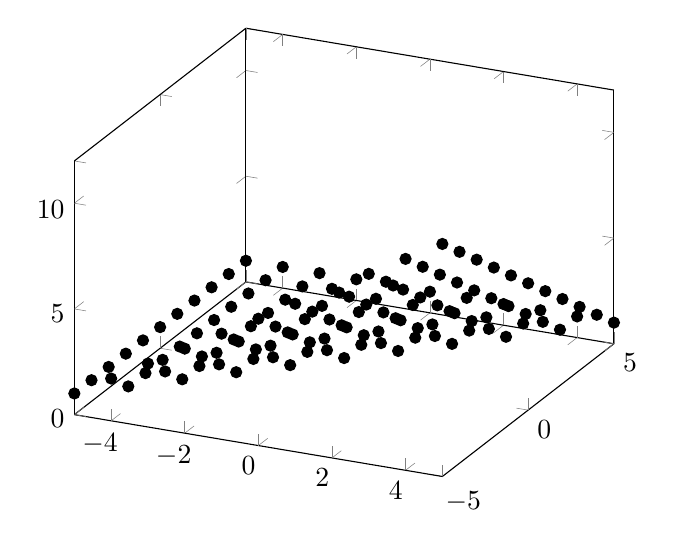
\begin{tikzpicture}
    \begin{axis}
      \addplot3 [
        unbounded coords=jump,
        mesh,
        shader=interp,
        samples at={-5,...,5},
        samples y={11},
        only marks,
      ] {1+max(x-y,0)};
    \end{axis}
  \end{tikzpicture}
  \hfil
  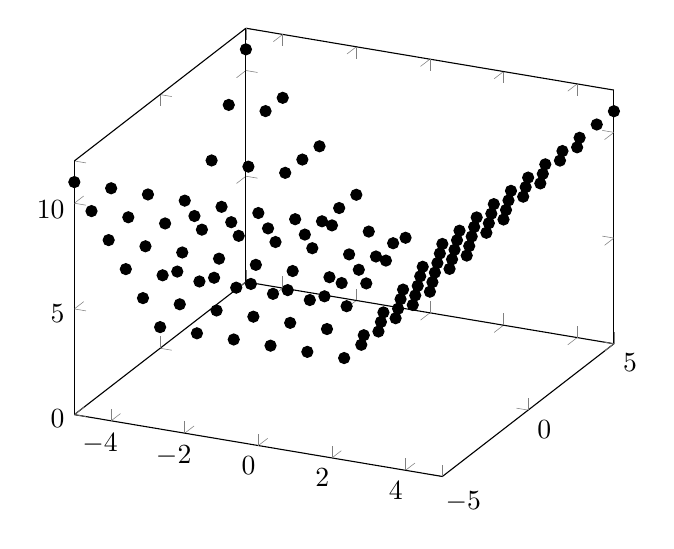
\begin{tikzpicture}
    \begin{axis}
      \addplot3 [
        unbounded coords=jump,
        mesh,
        shader=interp,
        samples at={-5,...,5},
        samples y={11},
        only marks,
      ] {1+abs(max(x,-y))+abs(max(x,-y))};
    \end{axis}
  \end{tikzpicture}
  \caption{Evaluation of the motivational example}
  \label{fig:motivational_evaluation}
\end{figure}

  As already pointed out, the polynomial $x-y$ is a time rank for the location $\location_1$.
  This fact can be formalized in the following way.
  Consider the function $\timerank: \LSet \rightarrow \BoundSet_p(\PVSet)$ with $\timerank(\location_1) = x-y$.
  This function is a time ranking function for the transition set $\TSet = \braced{t_1}$, if $\TSet_> = \braced{t_1}$.
  For the single transition $t_1$ it holds for every evaluation step $(\location_1,\valuation) \rightarrow_{t_1} (\location_1,\valuation')$ that $\exacteval{x>y}{\valuation} \Rightarrow \exacteval{x-y}{\valuation} > \exacteval{x-y}{\valuation'}$, since $x$ decreases such an evaluation step.
  Also, it holds for every evaluation step $(\location_1,\valuation) \rightarrow_{t_1} (\location_1,\valuation')$ that $\exacteval{x>y}{\valuation} \Rightarrow \exacteval{x-y}{\valuation} \geq 1$.
  Note that in this example it would also be possible to consider the transition $t_0$ as part of the set $\TSet$, since it holds for every evaluation step $(\location_1,\valuation) \rightarrow_{t_0} (\location_1,\valuation')$ that $\valuation(x)=\valuation'(x)$ and $\valuation(y)=\valuation'(y)$ and therefore $\exacteval{\textbf{true}}{\valuation} \Rightarrow \exacteval{x-y}{\valuation} \geq \exacteval{x-y}{\valuation'}$.
\end{example}

For the computation of ranking functions, it is common to use an SMT-Solver.
An SMT-Solver is capable of proving satisfiability and unsatisfiability of existential formulas.
The presented definition of time ranking functions and cost ranking functions consists of conditions, which need to be fulfilled for all states $\valuation, \valuation' \in \Valuation$ of all evaluation steps $(\location, \valuation) \rightarrow_t (\location', \valuation')$.
Such a universal quantified formula can be proven by showing the unsatisfiability of the negation of the formula with an SMT-Solver.
But for ranking functions it is also necessary to consider, that the coefficients of a timerank polynomial $\timerank(\location)$ are existentially quantified in the conditions of the ranking function definition.
Therefore, a negation of the condition yields universal quantification of the coefficients of a timerank.
Thus, the negation of the condition is also not provable by an SMT-Solver.

For such formulas, which contain both existential and universal quantification, it is common to use a variant of Farkas' lemma \cite{schrijver1998theory} specialized for polyranking \cite{bradley2005polyranking}.
For this purpose, it is necessary to restrict the domain of timeranks $\timerank(\location)$ and costranks $\costrank(\location)$ to affine polynomials $\BoundSet_a(\PVSet)$.
Then, it is possible to transform the problem of finding a ranking function into a problem solvable with an SMT-Solver.
